\begin{frame}[t]\label{a.3a}
\frametitle{Beyond the DF Theory}%Beyond the Dynamics-Based Perspective}%DF Theory}

\only<1-4>{
There are \textbf{three open questions} $\ldots$
}
\only<5->{
We think we got two out of the three (computing  $J_\sigma$ and $T_\mathrm{o}$ without fitting to relaxation data)!
}
\vspace{-1.5em}
\hspace{-1.5em}\begin{tabulary}{1.05\linewidth}{CCC}
\onslide<2->{\textbf{\Large Excitations}} &  \onslide<3->{\textbf{\Large Onset Temperature}} & \onslide<4->{\textbf{\Large Facilitation}} \\  
\onslide<2->{
\only<2-4>{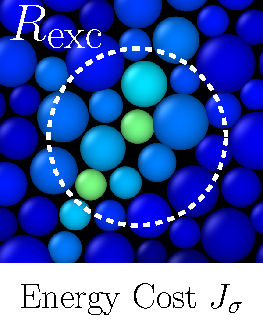
\includegraphics[height=0.3\textwidth]{a.2-intro_dftheory/DF_Theory_Excitations_Zoom.pdf}}
\only<5->{\begin{center}\textcolor{green!60!black}{\Huge ✓}\\\textbf{\small SOLVED}\end{center}}

} & \onslide<3->{
\only<3-4>{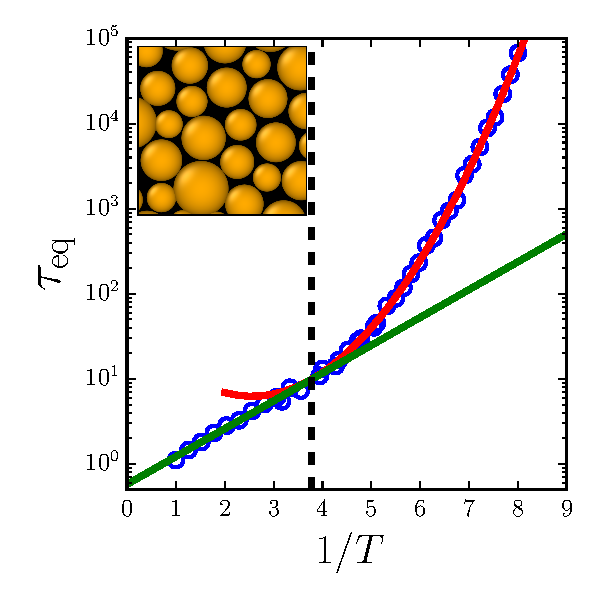
\includegraphics[height=0.3\textwidth]{intro_glassy/timerelax_poly12_4.pdf}
}
\only<5->{\begin{center}\textcolor{green!60!black}{\Huge ✓}\\\textbf{\small SOLVED}\end{center}}
} & \onslide<4->{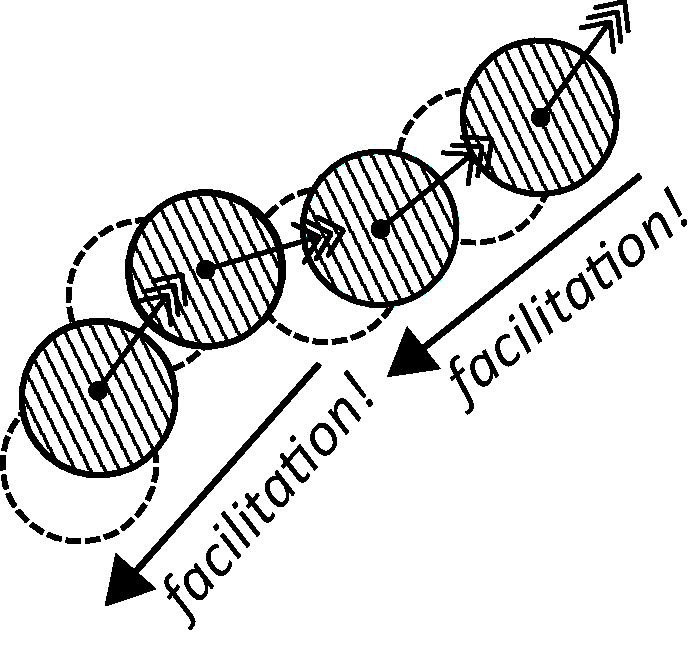
\includegraphics[height=0.3\textwidth]{a.2-intro_dftheory/facilitation_closer_2.pdf}} \\
\vspace{-1em}
\onslide<2->{
\only<2-4>{{\small What is the origin of "localized excitations" and their energy cost $J_\sigma$?}}
\only<5->{{\small  Hasyim, Mandadapu, \textit{J. Chem. Phys.} 155 (4), 44504 (2021)}}
} & 
\vspace{-1em}
\onslide<3->{
\only<3-4>{{\small Why do excitations emerge below an onset temperature $T_\mathrm{o}$?}}
\only<5->{{\small Fraggedakis, Hasyim, Mandadapu, \texttt{arXiv:2204.07528} (2022)}}
}
& 
\vspace{-1em}
\onslide<4->{{\small How does facilitation and $\tilde{\gamma}$ emerge from the glassy system?}} %\\
\end{tabulary}

\end{frame} 